%%%%%%
%BASE
%%%
\documentclass[12pt,landscape]{article}
\usepackage[a4paper]{geometry}
\usepackage[utf8]{inputenc}
\usepackage[T1]{fontenc}
\usepackage[francais]{babel}
\pagestyle{empty}

%%%%%
%MATHS
%%%
\usepackage{amsmath}
\usepackage{array}
\usepackage{multicol}

%%%%%
%COULEURS
%%%
\usepackage{xcolor}
\usepackage{color}
\usepackage{colortbl}


%%%%%
%IMAGES
%%%
\usepackage{ebgaramond} %
\usepackage{caption}
\usepackage{graphicx, threeparttable}
\usepackage{wrapfig}
\usepackage{graphicx}
\DeclareCaptionFormat{sanslabel}{#3}%


%%%%%
%PUCES
%%%
\usepackage{pifont}
\everymath{\displaystyle}
\usepackage{hyperref}
\setlength{\parindent}{10px}

%%%%%
%Tableau
%%%
% Permet d'agrandir le tableau.
\renewcommand{\arraystretch}{1.5}
\setlength{\tabcolsep}{0.5cm}

%%%%%
%Haut de Page
%%%
\usepackage{fancybox}
\usepackage{fancyhdr}
%\usepackage[left=5cm,right=5cm,top=6cm,bottom=7cm]{geometry}

\pagecolor[RGB]{105,110,103}
%\pagecolor[RGB]{248,157,48}


\begin{document}
\begin{center}
        %\shadowbox{
		\Huge
               \colorbox[RGB]{248,157,48}{ \textcolor{black}{AMAZON}}
        \normalsize
%}
    \end{center}
\begin{multicols}{2}
\begin{tabular}{l}
  %\hline
	  \rowcolor[RGB]{248,157,48} Pays d'origine : \'Etats-Unis \\
	  \rowcolor[RGB]{248,157,48} Date de création : 5 juillet 1994 \\
	  \rowcolor[RGB]{248,157,48}Le siège social actuel d'amazon est à Seatle aux \'Etats-Unis\\
	  \rowcolor[RGB]{248,157,48} Introduite en bourse en mai 1997\\
	  \rowcolor[RGB]{248,157,48} Secteur d'activité : Objets du quotidien, lingerie,\\
	  \rowcolor[RGB]{248,157,48} ~~~cosmétiques, appareil électronique,\\
	  \rowcolor[RGB]{248,157,48} ~~~accessoires de tout types, des produits alimentaires,\\
	  \rowcolor[RGB]{248,157,48} ~~~livres physiques et numérique.\\
	  \rowcolor[RGB]{248,157,48} Marques de l'entreprise : Tout types de marques,\\
      \rowcolor[RGB]{248,157,48} ~~~de la plus connue, à la moins connue. \\
	  \rowcolor[RGB]{248,157,48}Adresse du site internet : https://www.amazon.com/ \\
	  \rowcolor[RGB]{248,157,48} Le créateur d'amazon est Jeff bezos. \\
  %\hline
\end{tabular}
\begin{center}
~~~~~~~~~~~~~~~~~~~~~~~~~~~~~~~~~~~~~~~~~~~~~~~~~
\includegraphics[width=3cm]{120px-Amazon_icon.png}
\end{center}
\begin{tabular}{l}
  %\hline
 \rowcolor[RGB]{248,157,48}	  Nombre de salariés : 647.500\\
 \rowcolor[RGB]{248,157,48}	  Nombre de magasins : 3000 magasins comptent ouvir en 2021\\
 \rowcolor[RGB]{248,157,48}	  Sous-traitants : Tous les services de transports (Chronopost, DHL, Mondial Relay...) \\
 \rowcolor[RGB]{248,157,48}	  1.000 milliards de dollars capitalisation boursière \\
 \rowcolor[RGB]{248,157,48}	  Chiffre d'affaire : 177,9 milliards \$ \\
 % \hline
\end{tabular}
\end{multicols}
\begin{figure}[h]\captionsetup{format=sanslabel}
\begin{center}
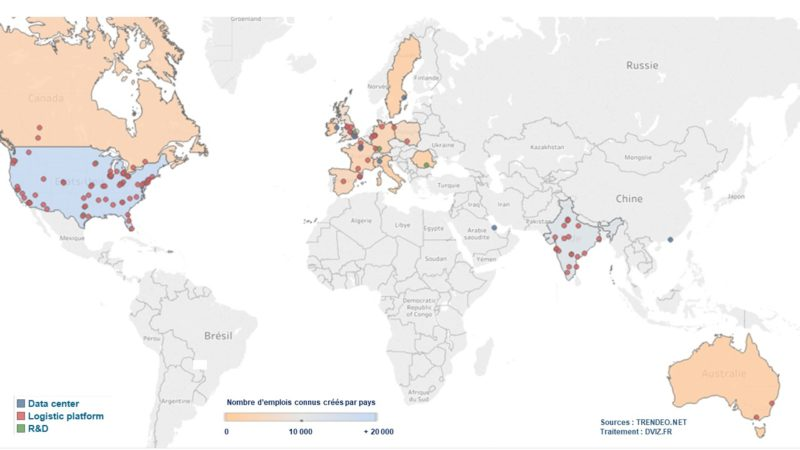
\includegraphics[width=15cm]{cate_2.jpg}
\caption{Implantations d'Amazon dans le monde}
\end{center}
\end{figure}
    \vspace{0.5 cm}
%\newpage
\begin{tabular}{l}
 % \hline
 \rowcolor[RGB]{248,157,48} Stratégie de développement :  En collaboration avec Hasbro, les emballages moins coûteux pour les achats en ligne. \\
 \rowcolor[RGB]{248,157,48} ~~~~Attractif pour les magasins et facile à ouvrir, recycler pour les achats en ligne.\\
 \rowcolor[RGB]{248,157,48} Investissements : Amazon s'est lancé dans la livraison en 24H pour les abonnés prime.\\
 \rowcolor[RGB]{248,157,48} Problèmes : \`A cause de ce lancement, Amazon s'est vu baisseer son chiffre d'affaire de 26\%.\\
 \rowcolor[RGB]{248,157,48} ~~~~B2S une société de livraison de colis amazon déménage pendant la nuit en raison de mauvaises condition de travail.\\
  %\hline
\end{tabular}
\vspace{0.5 cm}

\begin{tabular}{l}
 \rowcolor[RGB]{248,157,48} \textbf{\underline{\`A l'échelle locale:}}\\
\rowcolor[RGB]{248,157,48} Amazon ouvre son premier supermarché alimentaire sans caisse, Amazon Go.~~~~~~~~~~~~~~~~~~~~~~~~~~~~~~~~~~~~~~~~~~~~~~~~~~~~~~~~~
\includegraphics[width=3cm]{amazongo.png}\\ 
\rowcolor[RGB]{248,157,48}  Situé à Seattle, près du siège de l'entreprise, il reste en phase de test pendant près d'un an, réservé aux employés d'Amazon.\\
\rowcolor[RGB]{248,157,48} En janvier 2018, le magasin est ouvert au grand public\\
\rowcolor[RGB]{248,157,48}En juillet 2019, on compte 13 magasins Amazon Go aux États-Unis \\
\end{tabular}\\
\end{document}

